\chapter{Создание логической\\и физической модели данных}
\label{cha:dmd}

\section{Работа по методическим указаниям}
\subsection*{Теоретический материал}
На этапе {инфологического} проектирования базы данных должна быть построена
модель предметной области, не привязанная к конкретной СУБД, понятная не только
разработчикам информационной системы, но и экономистам, менеджерам и другим
специалистам. В то же время модель предметной области должна максимально точно
отражать семантику предметной области и позволять легко перейти к модели данных
конкретной СУБД.

\textbf{Логический уровень} --- это уровень, соответствующий \\инфологическому этапу проектирования
и не привязанный к конкретной СУБД. Модели логического уровня оперируют с
понятиями сущностей, атрибутов и связей, которые на этом уровне именуются на
естественном языке (в нашем случае – на русском) так, как они называются в
реальном мире.

\textbf{Физический уровень} --- это отображение логической модели на модель данных
конкретной СУБД. Одной логической модели может соответствовать несколько
физических моделей. Причем, Erwin (как и другие CASE-системы проектирования баз
данных) позволяет автоматизировать отображение логической модели на физическую.

%Модель <<сущность-связь>> строится в виде диаграммы <<сущность-связь>>,
%основными компонентами которой являются сущности (Entity) и связи\\(Relationship).
%Отсюда происходят часто используемые названия модели (ER-модель) и диаграммы
%(ER-диаграмма).

В ходе данной практической работы нами была описана и построена логическая и физическая модель данных средствами ПО \erdatamodaler.

Порядок построения модели данных в среде \textbf{ERwin} рассмотрим на примере
автоматизированной информационной системы "Реализация средств вычислительной
техники", предназначенной для учета продаж настольных компьютеров по заказам
клиентов.

Создание модели данных начинается с разработки логической модели, которая
должна представлять состав сущностей предметной области с перечнем атрибутов и
отношений между ними.

%В зависимости от глубины представления информации о данных различают 3
%подуровня логического уровня модели данных:
%\begin{itemize}
%	\item  диаграмма сущность – связь \texttt{(Entity Relationship Diagram, ERD)};
%	\item модель данных, основанная на ключах (\texttt{Key Based model, KB)}; --- полная атрибутивная модель данных \texttt{(Fully Attributed model, FA)}.
%\end{itemize}
%
%\texttt{Диаграмма сущность-связь} включает сущности и взаимосвязи, отражающие
%основные бизнес-правила предметной области.
%
%\texttt{Модель данных, основанная на ключах} --- более подробное представление данных.
%Данная модель включает описание всех сущностей и первичных ключей,
%необходимых для подробного описания предметной области.
%
%\texttt{Полная атрибутивная модель данных} --- наиболее детальное представление
%структуры данных предметной области. Данная модель представляет данные в третьей
%нормальной форме и включает все сущности, атрибуты и связи.
%
%Логическим соотношением между сущностями является \textbf{связь}. Каждому виду
%связи соответствует определенная кнопка, расположенная на палитре инструментов.
%Имя связи выражает некоторое ограничение или правило и облегчает чтение
%диаграммы. Каждая связь должна именоваться глаголом или глагольной фразой.

Результат разработки логической модели данных системы <<Реализация средств
вычислительной техники>>, предназначенной для учета продаж настольных
компьютеров по заказам клиентов приведен на Рисунке \ref{fig:2-logical-model-method}.

% TODO: \usepackage{graphicx} required
\begin{figure}[htpb]
	\centering
	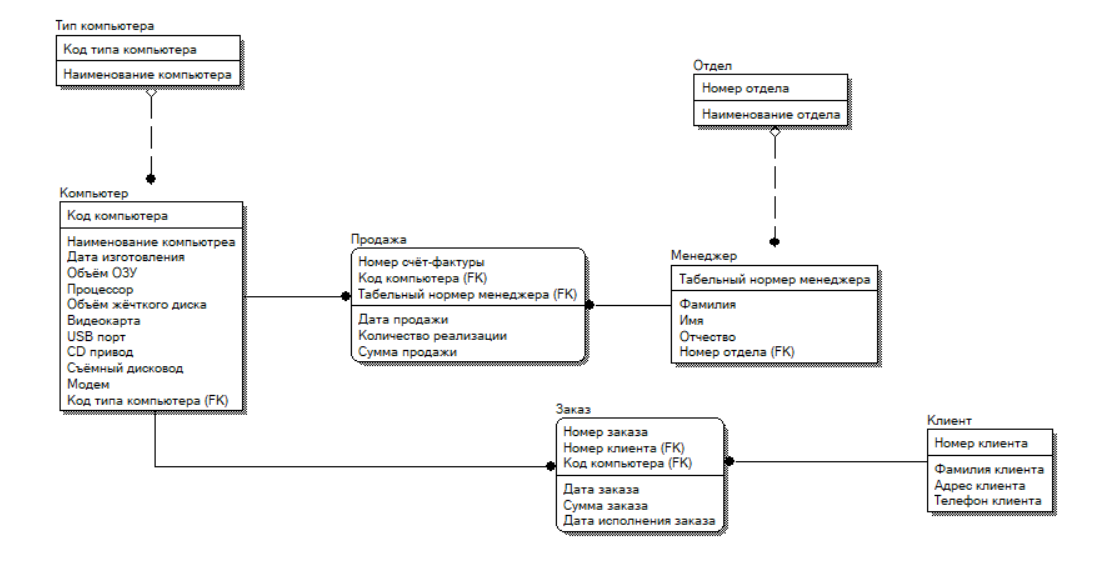
\includegraphics[width=0.7\linewidth]{images/2-method}
	\caption{Логическая модель данных системы <<Реализация средств вычислительной техники>>}
	\label{fig:2-logical-model-method}
\end{figure}

Для построения физической модели данных системы, следует определиться с СУБД, в которой будет реализована модель. При построении физической модели данных следует учитывать формальную теория представления и обработки данных в конкретной системе управления базами данных (СУБД).

В данной практической работе в качестве СУБД выбрана MySQL.

Приступим к построению физической модели данных системы <<Реализация средств вычислительной техники>>. Результат работы можно видеть на Рисунке \ref{fig:2-phisical-model}.

% TODO: \usepackage{graphicx} required
\begin{figure}[h!]
	\centering
	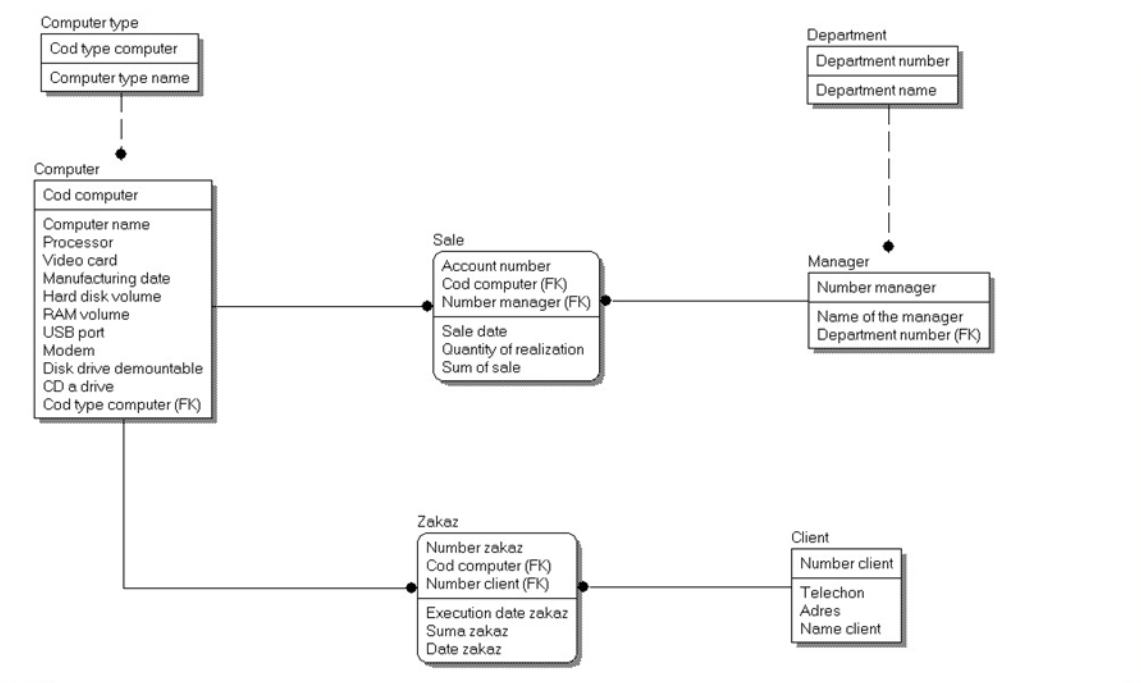
\includegraphics[width=0.7\linewidth]{images/2-phisical-model}
	\caption{Физическая модель данных системы <<Реализация средств вычислительной техники>>}
	\label{fig:2-phisical-model}
\end{figure}
\newpage
\subsection{\individual}
Приступим к построению логической модели данных системы <<Велосипедное предприятие>>. 
В соответствии с моделью, реализованной в ходе первой практической работы, добавим в рабочую область следующие сущности:
\begin{itemize}
	\item Component;
	\item FrameInfo;
	\item Frame;
	\item Frameset;
	\item FrameSize;
	\item Fork;
	\item ComponentType;
	\item Wheelset;
	\item Groupset;
	\item Brake;
	\item FctCycleBuild;
	\item CycleType;
	\item Bar;
	\item Setup.
\end{itemize}
Добавим связи между сущностями в соответствии с ранее построенной моделью. Логическая модель системы <<Велосипедное предприятие>> приведена на Рисунке \ref{fig:2-cycle-logical}.

% TODO: \usepackage{graphicx} required
\begin{figure}[h!]
	\centering
	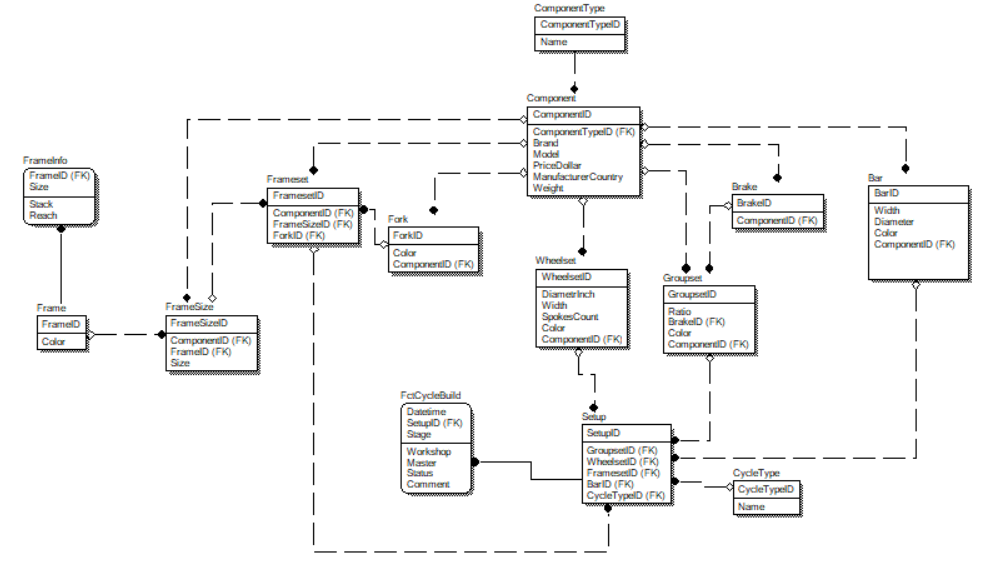
\includegraphics[width=0.8\linewidth]{images/2-cycle-logical}
	\caption{Логическая модель данных системы <<Велосипедное предприятие>>}
	\label{fig:2-cycle-logical}
\end{figure}

После уточнения типов данных, выбранных в соответствии с предметной областью и спецификой СУБД MySQL.
Физическая модель системы <<Велосипедное предприятие>> приведена на Рисунке \ref{fig:2-cycle-phisical}.

% TODO: \usepackage{graphicx} required
\begin{figure}[h!]
	\centering
	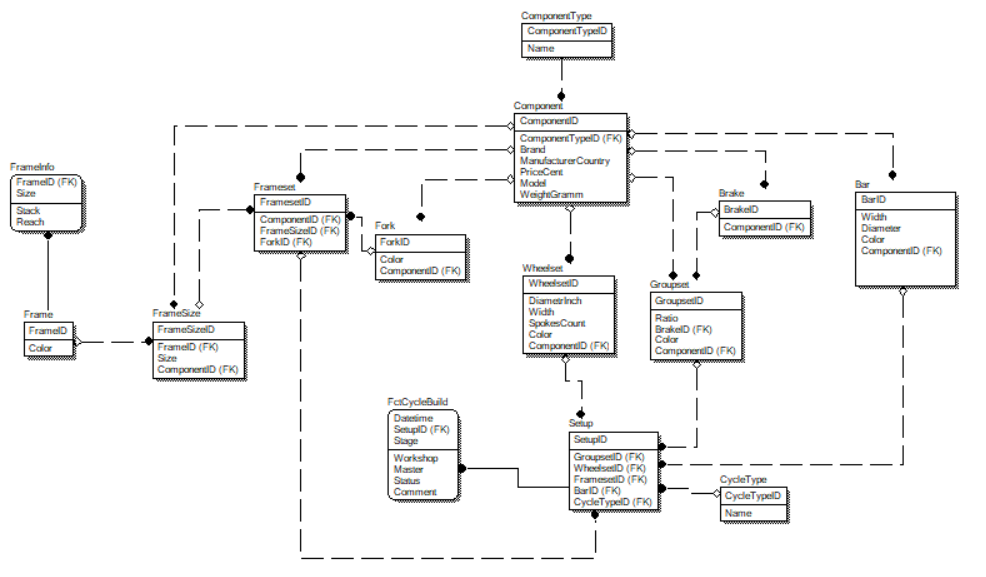
\includegraphics[width=0.8\linewidth]{images/2-cycle-phisical}
	\caption{Физическая модель данных системы <<Велосипедное предприятие>>}
	\label{fig:2-cycle-phisical}
\end{figure}

После реализации физической и логической модели можно приступать к реализации модели данной системы в СУБД MySQL.
\hfill